% Created by tikzDevice version 0.12.5 on 2023-08-17 16:52:11
% !TEX encoding = UTF-8 Unicode
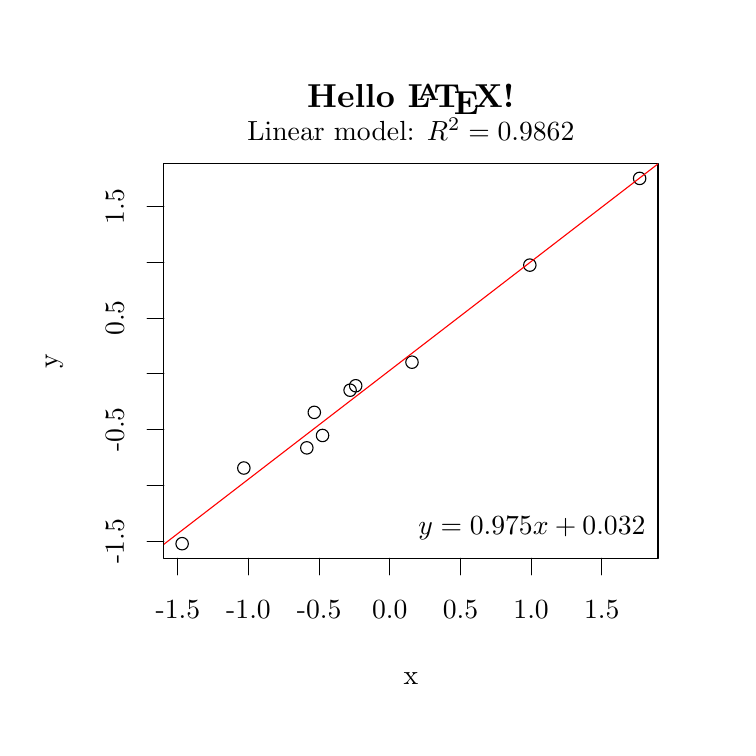
\begin{tikzpicture}[x=1pt,y=1pt]
\definecolor{fillColor}{RGB}{255,255,255}
\path[use as bounding box,fill=fillColor,fill opacity=0.00] (0,0) rectangle (252.94,252.94);
\begin{scope}
\path[clip] ( 49.20, 61.20) rectangle (227.75,203.75);
\definecolor{drawColor}{RGB}{0,0,0}

\path[draw=drawColor,line width= 0.4pt,line join=round,line cap=round] (106.55,105.58) circle (  2.25);

\path[draw=drawColor,line width= 0.4pt,line join=round,line cap=round] ( 78.11, 93.82) circle (  2.25);

\path[draw=drawColor,line width= 0.4pt,line join=round,line cap=round] (116.50,121.94) circle (  2.25);

\path[draw=drawColor,line width= 0.4pt,line join=round,line cap=round] ( 55.81, 66.48) circle (  2.25);

\path[draw=drawColor,line width= 0.4pt,line join=round,line cap=round] (181.45,167.14) circle (  2.25);

\path[draw=drawColor,line width= 0.4pt,line join=round,line cap=round] (100.87,101.10) circle (  2.25);

\path[draw=drawColor,line width= 0.4pt,line join=round,line cap=round] (103.57,113.93) circle (  2.25);

\path[draw=drawColor,line width= 0.4pt,line join=round,line cap=round] (118.53,123.54) circle (  2.25);

\path[draw=drawColor,line width= 0.4pt,line join=round,line cap=round] (138.87,132.06) circle (  2.25);

\path[draw=drawColor,line width= 0.4pt,line join=round,line cap=round] (221.13,198.47) circle (  2.25);
\end{scope}
\begin{scope}
\path[clip] (  0.00,  0.00) rectangle (252.94,252.94);
\definecolor{drawColor}{RGB}{0,0,0}

\path[draw=drawColor,line width= 0.4pt,line join=round,line cap=round] ( 54.28, 61.20) -- (207.44, 61.20);

\path[draw=drawColor,line width= 0.4pt,line join=round,line cap=round] ( 54.28, 61.20) -- ( 54.28, 55.20);

\path[draw=drawColor,line width= 0.4pt,line join=round,line cap=round] ( 79.81, 61.20) -- ( 79.81, 55.20);

\path[draw=drawColor,line width= 0.4pt,line join=round,line cap=round] (105.33, 61.20) -- (105.33, 55.20);

\path[draw=drawColor,line width= 0.4pt,line join=round,line cap=round] (130.86, 61.20) -- (130.86, 55.20);

\path[draw=drawColor,line width= 0.4pt,line join=round,line cap=round] (156.39, 61.20) -- (156.39, 55.20);

\path[draw=drawColor,line width= 0.4pt,line join=round,line cap=round] (181.92, 61.20) -- (181.92, 55.20);

\path[draw=drawColor,line width= 0.4pt,line join=round,line cap=round] (207.44, 61.20) -- (207.44, 55.20);

\node[text=drawColor,anchor=base,inner sep=0pt, outer sep=0pt, scale=  1.00] at ( 54.28, 39.60) {-1.5};

\node[text=drawColor,anchor=base,inner sep=0pt, outer sep=0pt, scale=  1.00] at ( 79.81, 39.60) {-1.0};

\node[text=drawColor,anchor=base,inner sep=0pt, outer sep=0pt, scale=  1.00] at (105.33, 39.60) {-0.5};

\node[text=drawColor,anchor=base,inner sep=0pt, outer sep=0pt, scale=  1.00] at (130.86, 39.60) {0.0};

\node[text=drawColor,anchor=base,inner sep=0pt, outer sep=0pt, scale=  1.00] at (156.39, 39.60) {0.5};

\node[text=drawColor,anchor=base,inner sep=0pt, outer sep=0pt, scale=  1.00] at (181.92, 39.60) {1.0};

\node[text=drawColor,anchor=base,inner sep=0pt, outer sep=0pt, scale=  1.00] at (207.44, 39.60) {1.5};

\path[draw=drawColor,line width= 0.4pt,line join=round,line cap=round] ( 49.20, 67.36) -- ( 49.20,188.29);

\path[draw=drawColor,line width= 0.4pt,line join=round,line cap=round] ( 49.20, 67.36) -- ( 43.20, 67.36);

\path[draw=drawColor,line width= 0.4pt,line join=round,line cap=round] ( 49.20, 87.52) -- ( 43.20, 87.52);

\path[draw=drawColor,line width= 0.4pt,line join=round,line cap=round] ( 49.20,107.67) -- ( 43.20,107.67);

\path[draw=drawColor,line width= 0.4pt,line join=round,line cap=round] ( 49.20,127.83) -- ( 43.20,127.83);

\path[draw=drawColor,line width= 0.4pt,line join=round,line cap=round] ( 49.20,147.98) -- ( 43.20,147.98);

\path[draw=drawColor,line width= 0.4pt,line join=round,line cap=round] ( 49.20,168.14) -- ( 43.20,168.14);

\path[draw=drawColor,line width= 0.4pt,line join=round,line cap=round] ( 49.20,188.29) -- ( 43.20,188.29);

\node[text=drawColor,rotate= 90.00,anchor=base,inner sep=0pt, outer sep=0pt, scale=  1.00] at ( 34.80, 67.36) {-1.5};

\node[text=drawColor,rotate= 90.00,anchor=base,inner sep=0pt, outer sep=0pt, scale=  1.00] at ( 34.80,107.67) {-0.5};

\node[text=drawColor,rotate= 90.00,anchor=base,inner sep=0pt, outer sep=0pt, scale=  1.00] at ( 34.80,147.98) {0.5};

\node[text=drawColor,rotate= 90.00,anchor=base,inner sep=0pt, outer sep=0pt, scale=  1.00] at ( 34.80,188.29) {1.5};

\path[draw=drawColor,line width= 0.4pt,line join=round,line cap=round] ( 49.20, 61.20) --
	(227.75, 61.20) --
	(227.75,203.75) --
	( 49.20,203.75) --
	cycle;
\end{scope}
\begin{scope}
\path[clip] (  0.00,  0.00) rectangle (252.94,252.94);
\definecolor{drawColor}{RGB}{0,0,0}

\node[text=drawColor,anchor=base,inner sep=0pt, outer sep=0pt, scale=  1.20] at (138.47,224.20) {\bfseries Hello \LaTeX!};

\node[text=drawColor,anchor=base,inner sep=0pt, outer sep=0pt, scale=  1.00] at (138.47, 15.60) {x};

\node[text=drawColor,rotate= 90.00,anchor=base,inner sep=0pt, outer sep=0pt, scale=  1.00] at ( 10.80,132.47) {y};
\end{scope}
\begin{scope}
\path[clip] ( 49.20, 61.20) rectangle (227.75,203.75);
\definecolor{drawColor}{RGB}{255,0,0}

\path[draw=drawColor,line width= 0.4pt,line join=round,line cap=round] ( 49.20, 66.25) -- (227.75,203.71);
\end{scope}
\begin{scope}
\path[clip] (  0.00,  0.00) rectangle (252.94,252.94);
\definecolor{drawColor}{RGB}{0,0,0}

\node[text=drawColor,anchor=base,inner sep=0pt, outer sep=0pt, scale=  1.00] at (138.47,212.14) {Linear model: $R^{2}= 0.9862 $};
\end{scope}
\begin{scope}
\path[clip] ( 49.20, 61.20) rectangle (227.75,203.75);
\definecolor{drawColor}{RGB}{0,0,0}

\node[text=drawColor,anchor=base west,inner sep=0pt, outer sep=0pt, scale=  1.00] at (141.16, 69.76) {$y = 0.975x +0.032$};
\end{scope}
\end{tikzpicture}
